\pagestyle{empty} % Limpa o cabeçalho e o rodapé
\onehalfspacing % Espaçamento entre-linhas de 1,5
% \hyphenpenalty=10000 % To prevent hyphenation
\pretolerance=10000 % To avoif overful lines
%\selectlanguage{english}
\setcounter{ex}{0} % counter for exercises
\selectlanguage{brazilian}
%\pagenumbering{arabic} % Uncomment this line if you want renumber pages for each chapter
\renewcommand{\chaptername}{Tutorial}
\chapter{Introdução ao TNT}\label{tut4}
\rhead{\tiny Instituto de Biociências --USP: BIZ0433 - Inferência Filogenética: Filosofia, Método e Aplicações}
\cfoot{\tiny \cc \ccby \ccsa \href{http://creativecommons.org/licenses/by-sa/4.0/}{Creative Commons Attribution-ShareAlike 4.0 International License}}
%\vspace{5pt}
{\large \sc BIZ0433 - Inferência Filogenética: Filosofia, Método e Aplicações.}\par
%\vspace{10pt}
\par
\minitoc % for table of contents within the chapter
\newpage
\section*{}\addcontentsline{toc}{section}{Objetivo}
\onehalfspacing
\vspace*{5pt}
\begin{center}
\emph{\begin{large}Objetivo\end{large}}\label{tut4:Objetivo}
\vspace{2pt}
\end{center}
%% TEXTO DO RESUMO
O objetivo deste tutorial é introduzir conceitos básicos associados ao uso do TNT. Este aplicativo é um dos mais versáteis e rápidos disponíveis para a busca de árvores filogenéticas utilizando parcimônia como critério de otimalidade. Neste tutorial iremos explorar a sintaxe dos arquivos de entrada deste programa para matrizes e topologias, verificar como TNT salva as topologias encontradas e entender como o TNT executa buscas exaustivas e heurísticas. Os arquivos associados a este tutorial estão disponíveis em \url{http://lhe.ib.usp.br/cladistica}. Você pode baixá-los diretamente com o seguinte comando:

\begin{center}
\small \texttt{wget http://lhe.ib.usp.br/downloads/tutorial\_04.zip}\\
\end{center}

\newpage
\pagestyle{fancy} % Inclui o cabeçalho definido no meta.tex
%\pagenumbering{arabic} % Números das páginas em arábicos
\begin{refsection}
\renewcommand*{\finalnamedelim}{\addspace\&\space}% Usar '&' ao invés de 'e'.

%%%%%%%%%%%%%%%%%%%%%%%%%%%% HERE TEXT STARTS %%%%%%%%%%%%%%%%%%%%%%%%%%%% 
\section{Considerações gerais}\label{tut4:general}

	O TNT \parencite{GoloboffEtAl_2008} é um programa para inferência filogenética que utiliza parcimônia como critério de otimalidade na buscas de topologias com menor custo. O programa permite a análise de dados morfológicos discretos e contínuos, bem como de dados genotípicos concatenados ou em partições distintas. Há duas distribuições básicas de TNT. Uma para o sistema operacional Windows, que possui interface gráfica, e outra para Linux/Mac OS X, que deve ser executada por comandos de linha. Neste tutorial, iremos utilizar a versão sem interface gráfica, pois ela é mais versátil, principalmente quando você deseja fazer uma série de análises cuja implementação pode ser feita por meio de \textit{scripts}. Esse tutorial assume que você possui o TNT instalado em seu computador. Caso seja necessário instalá-lo, baixe a versão compatível com seu sistema operacional na página \url{http://www.lillo.org.ar/phylogeny/tnt/}.

\section{Estrutura dos arquivos de entrada}\label{tut4:input}
	A estrutura mais simples de um arquivo de entrada para TNT obedece a seguinte formatação:
\\
\indent\indent\texttt{xread}\\
\indent\indent\texttt{'qualquer comentário'}\\
\indent\indent\texttt{No.\_de\_caracteres  No.\_de\_taxóns}\\
\indent\indent\texttt{taxon\_1   dados}\\
\indent\indent\texttt{taxon\_2   dados}\\
\indent\indent\texttt{…}\\
\indent\indent\texttt{taxon\_n   dados}\\
\indent\indent\texttt{;}\\

Para dados morfológicos discretos essa matriz seria:
\\
\indent\indent\texttt{xread}\\
\indent\indent\texttt{'dados morfologicos'}\\
\indent\indent\texttt{5  4}\\
\indent\indent\texttt{taxon\_1   00010}\\
\indent\indent\texttt{taxon\_2   10000}\\
\indent\indent\texttt{taxon\_3   11001}\\
\indent\indent\texttt{taxon\_4   11100}\\
\indent\indent\texttt{;}\\

Para dados moleculares usaríamos:
\\
\indent\indent\texttt{nstates dna;}\\
\indent\indent\texttt{xread}\\
\indent\indent\texttt{'formato para dados moleculares'}\\
\indent\indent\texttt{8 6}\\
\indent\indent\texttt{taxon\_1 ACGTACGT}\\
\indent\indent\texttt{taxon\_2 AAGTACGT}\\
\indent\indent\texttt{taxon\_3 AAATACGT}\\
\indent\indent\texttt{taxon\_4 AAAAACGT}\\
\indent\indent\texttt{taxon\_5 AAAAAAGT}\\
\indent\indent\texttt{taxon\_6 AAAAAAAT}\\
\indent\indent\texttt{;}\\

Note que, para dados moleculares, a instrução dada ao TNT é expressa na primeira linha do arquivo de entrada -- onde se lê ``\texttt{nstates dna;}''.\\

Você pode ainda combinar dados genotípicos e fenotípicos utilizando uma estrutura como esta:
\\
\indent\indent\texttt{nstates 32}\\
\indent\indent\texttt{xread}\\
\indent\indent\texttt{14 5}\\
\indent\indent\texttt{\& [dna]}\\
\indent\indent\texttt{A ACCCCTGT}\\
\indent\indent\texttt{B ACCCCTGT}\\
\indent\indent\texttt{C NCCCCTGT}\\
\indent\indent\texttt{D ACCCCTGA}\\
\indent\indent\texttt{E ACCCCTGA}\\
\indent\indent\texttt{\& [prot]}\\
\indent\indent\texttt{A  KKKQ}\\
\indent\indent\texttt{B  KKKQ}\\
\indent\indent\texttt{C  KKKQ}\\
\indent\indent\texttt{D  KKKI}\\
\indent\indent\texttt{E  KKKI}\\
\indent\indent\texttt{\& [num]}\\
\indent\indent\texttt{A  00}\\
\indent\indent\texttt{B  11}\\
\indent\indent\texttt{C  12}\\
\indent\indent\texttt{D  12}\\
\indent\indent\texttt{E  13}\\
\indent\indent\texttt{;}\\

Neste último caso, o termo ``\texttt{nstates 32}'' define o número máximo de estados de caráter que o TNT deverá considerar, e os termos  ``\texttt{\& [dna]}'',  ``\texttt{\& [prot]} e  ``\texttt{\& [num]}'' definem cojuntos de dados para nucleotídeos, proteínas e numéricos, respectivamente.

Seguindo essas estruturas, você poderá usar qualquer editor de texto simples (i.e., word pad, gedit e textedit, entre outros) para escrever qualquer matriz a ser usada pelo TNT. Independetemente do editor escolhido, é importante que o arquivo seja salvo em formato texto, caso contrário o editor irá inserir caracteres ocultos que impedirão o TNT de ler o documento. Há editores de matrizes, tais como \href{http://www.mesquiteproject.org/}{Mesquite} -- que funciona em todas as plataformas e \href{http://en.bio-soft.net/tree/NDE.html}{NEXUS} -- exclusivamente para WINDOWS. Para o propósito de entender como o TNT funciona não será necessário utilizar esses aplicativos, mas é bom que vocês saibam que eles existem, pois os mesmos podem ser úteis para desenvolver projetos mais complexos para os quais você deseja anotar dados adicionais relacionados às definições de caracteres e estados de caráter.\\


\stepcounter{ex}
\begin{blackBlock}{\textbf{Exercicio 4.\arabic{ex}}}\label{tut4:ex:4.1}
	Em um teminal, você devera examinar o conteúdo arquivo ``\texttt{matriz\_1.tnt}'' do diretório  ``\texttt{tutorial\_4}'' utilizando comandos de linha ou editores de sua escolha. Correlacione o conteúdo deste arquivo com as estruturas apresentadas acima. A primeira linha deste arquivo (``\texttt{xread}'') informa ao TNT que ele deve ler uma matriz de dados. Na segunda linha, há um comentário (\textit{i.e.}, \texttt{'essa eh sua primeira matrix'}) que será impresso no terminal quando o TNT ler a matrix. A terceira linha (``\texttt{1 6}) informa ao programa que essa matriz possui uma coluna de caractéres e seis linhas de terminais. Posteriormente, você encontra a matriz de dados propriamente dita, e finalmente um ``\texttt{;}'' que indica ao TNT que a matriz terminou.

\begin {myindentpar}{0.5cm}
\begin{enumerate}[\itshape i.]
	\item{Você deverá criar uma arquivo chamado ``\texttt{exemplo\_1.tnt}'' que contenha os dados abaixo e no formato que possa ser lido pelo TNT.}\label{tut4:input:ex1:matriz}

	\item{Ao lado, você deverá desenhar a topologia mais parcimoniosa para esta matriz.}\label{tut4:input:ex1:tree_manual}\\

\end{enumerate}
\end{myindentpar}
\end{blackBlock}

\begin{table}[H]
\begin{tabular}{|l|l|}
\hline
 & \\
~~~~~~\texttt{taxon\_1 00000}~~~~~~ & ~~~~~~~~~~~~~~~~~~~~~~~~~~~~~~~~~~~~~~ \\
~~~~~~\texttt{taxon\_2 10000}~~~~~~ & ~~~~~~~~~~~~~~~~~~~~~~~~~~~~~~~~~~~~~~ \\
~~~~~~\texttt{taxon\_3 11000}~~~~~~ & ~~~~~~~~~~~~~~~~~~~~~~~~~~~~~~~~~~~~~~ \\
~~~~~~\texttt{taxon\_4 11100}~~~~~~ & ~~~~~~~~~~~~~~~~~~~~~~~~~~~~~~~~~~~~~~ \\
~~~~~~\texttt{taxon\_5 11110}~~~~~~ & ~~~~~~~~~~~~~~~~~~~~~~~~~~~~~~~~~~~~~~ \\
~~~~~~\texttt{taxon\_6 11101}~~~~~~ & ~~~~~~~~~~~~~~~~~~~~~~~~~~~~~~~~~~~~~~ \\
 & \\\hline
\end{tabular}
\end{table}




Antes de seguirmos à diante, veremos se o TNT está lendo o arquivo ``\texttt{exemplo\_1.tnt}'' -- ou seja, verificaremos se o arquivo não possuí nenhum erro se sintaxe. A primeira coisa de devemos fazer é executar o TNT. No \textit{prompt} do seu terminal execute:\\
\indent\indent\indent\shellcmd{ tnt}\\

Você deferá obter o \textit{prompt} de iniciação do TNT ilustrado na Figura \ref{tut4:fig:tnt1}:\\

%%%%%%%%%%%%%%%%%%%%%%%%%%% FIGURA TNT %%%%%%%%%%%%%%%%%%%%%%%%%%%
%  \vspace{-1em}
  \begin{figure}[H]
    %\ffigbox[\FBwidth]
       \centering
      {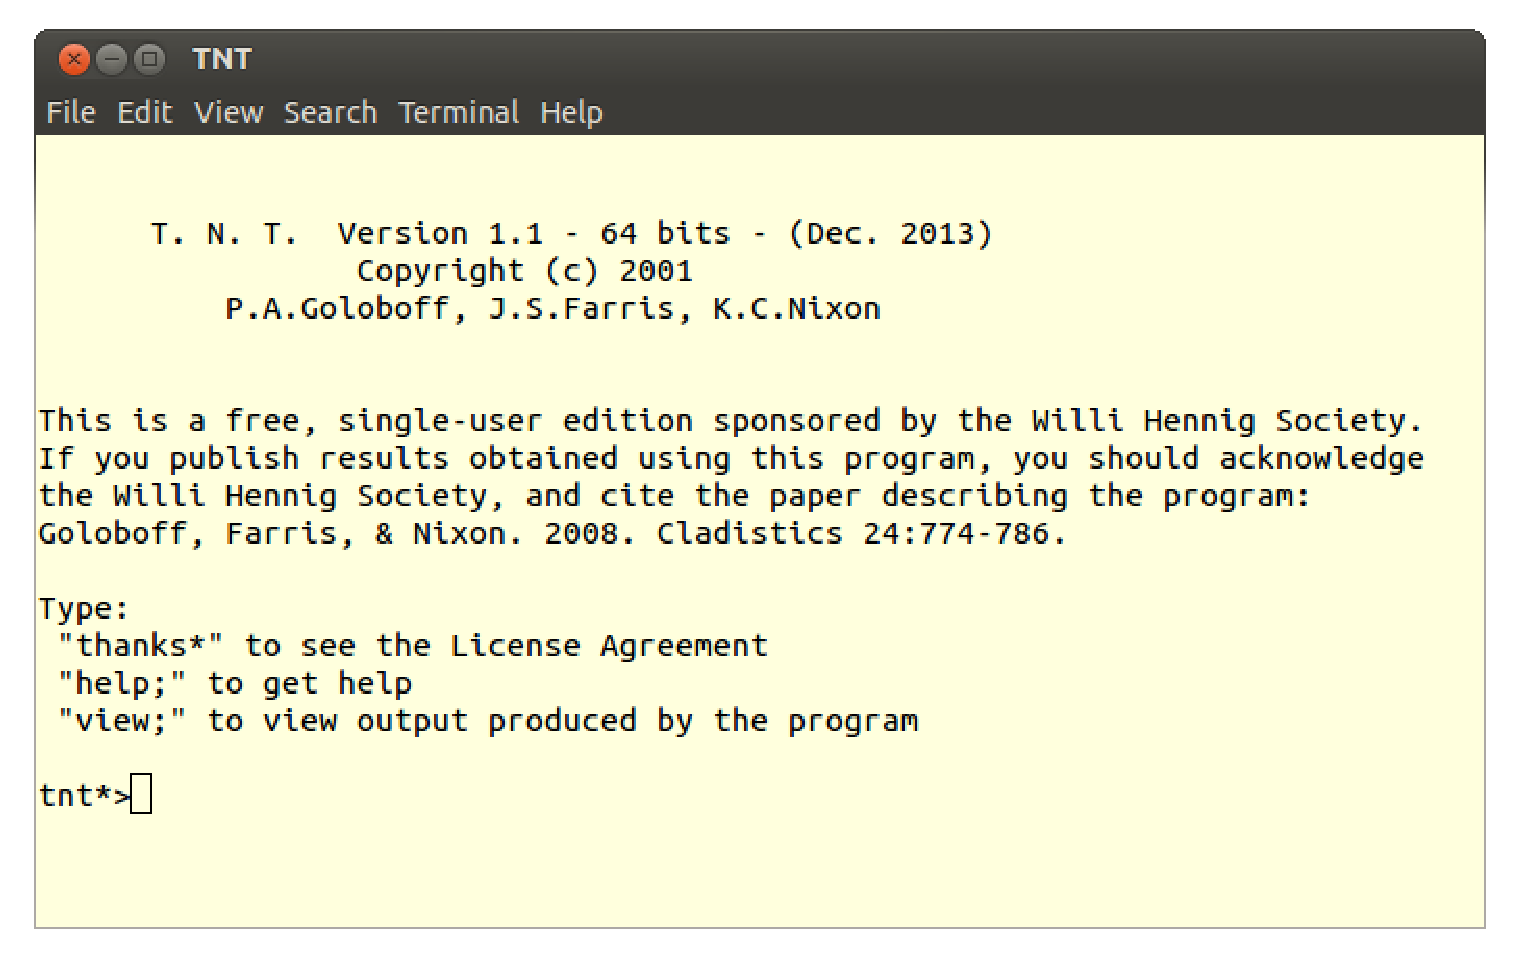
\includegraphics[scale=0.60]{figures/tut4/tnt_1.eps}}
      {\caption[\textit{\textit{Prompt de TNT} }]{\textit{Prompt} de iniciação do TNT.}\label{tut4:fig:tnt1}}
  \end{figure}

%%%%%%%%%%%%%%%%%%%%%%%%%%% FIM DA FIGURA TNT %%%%%%%%%%%%%%%%%%%%%

O comando de leitura de arquivos no TNT é ``\texttt{proc}'', de \textit{procedure}. Todos os comandos em TNT devem ser seguidos de ``\texttt{;}''. Se você digitar ``\texttt{help proc;}'' você obterá:
\\
\indent\indent\texttt{tnt*>help proc;}\\
\\
\indent\indent\texttt{PROCEDURE}\\
\indent\indent\indent\texttt{Redirect input }\\
\indent\indent\indent\texttt{XXX;~~~take commands from file XXX }\\
\indent\indent\indent\texttt{/;~~~~~close input file (include at end of file) }\\
\indent\indent\indent\texttt{...}\\
\\
portanto, para que o TNT leia o arquivo ``\texttt{exemplo\_1.tnt}'', basta você executar o seguinte comando:\\

\indent\indent\texttt{tnt*> proc exemplo\_1.tnt;}\\

o TNT deverá retornar:
\\
\indent\indent\texttt{Reading from exemplo\_1.tnt}\\
\indent\indent\texttt{Matrix (5x6, 16 states). Memory required for data:~~~0.02 Mbytes}\\

Caso você não tenha obtido o resultado acima, você deverá tentar identificar o erro e tentar  fazer com que o TNT leia seu arquivo de entrada novamente.

\section{Topologias em TNT}\label{tut4:input}
Obter topologias em programas de inferência filogenética é relativamente fácil; basta saber a sintaxe do(s) arquivo(s) de entrada e alguns comandos de execução. No entanto, entender como esses aplicativos tratam seus dados, quais são os tipos de análises disponíveis e como proceder para ter certeza de que você fez o que queria e explorou seus dados de maneira adequada requer um pouco mais do que simplesmente executar alguns comandos. Isso vale para comandos de linha e/ou análises em que você seleciona opções nos menus do programa.

Veja como é fácil obter uma topologia a partir do momento em que o TNT leu seu arquivo de entrada. Após ler o arquivo \texttt{``exemplo\_1.tnt''}, se você executar o  comando:\\

\indent\indent\texttt{tnt*> ie;}\\

Você deverá obter:
\\
\indent\indent\texttt{Implicit enumeration, 1 trees found, score 5.}\\

A mensagem de saída de TNT descreve o algorítmo utlizado na busca (\textit{i.e.}, ``Implicit enumeration''), número de topologia(s) encontrada(s) (\textit{i.e.}, ``1 trees found'') e o custo -- número de transformações -- desta(s) topologia(s) (\textit{i.e.}, ``score 5''). Para visualizar a topologia encontrada pelo TNT basta executar o seguinte comando:\\

\indent\indent\texttt{tnt*> tplot;}\\

Observe que o TNT utiliza o primeiro terminal de sua matriz como raíz caso nenhum outro seja especificado. Verifique o resultado impresso pelo TNT no terminal e responda:


\stepcounter{ex}
\begin{blackBlock}{\textbf{Exercicio 4.\arabic{ex}}}\label{tut4:ex:4.2}
	A topologia apresentada é a mesma que você obteve no exercício 4.1? No que elas diferem?
\vspace{90pt}
 \begin{center}
  \line(1,0){400}\\
  \line(1,0){400}\\
 \end{center}

\end{blackBlock}

Vamos repetir a busca novamente, mas antes disso iremos executar o comando ``\texttt{collapse [;}''. Após executá-lo, faça uma nova busca usando ``\texttt{ie;}'' e imprima a topologia no terminal. Essa nova topologia deve ser a mesma que você obteve manualmente. Por que isso acontece? Por \textit{default} o TNT irá sempre lhe fornecer \textbf{topologias binárias}, \textit{i.e.}, totalmente resolvidas ou dicotômicas, mesmo quando não existem caracteres sustentando um determinado nó. Portanto, \textbf{muito cuidado}! Muitas pessoas ignoram este componente da configuração do TNT e registram resultados irreais. Uma forma de evitar isso é sempre inserir o termo ``\texttt{collapse [;}'' no próprio arquivo de TNT, como no exemplo abaixo:
\\
\indent\indent\indent\texttt{xread}\\
\indent\indent\indent\texttt{5 6}\\
\indent\indent\indent\texttt{taxon\_1 00000}\\
\indent\indent\indent\texttt{taxon\_2 10000}\\
\indent\indent\indent\texttt{taxon\_3 11000}\\
\indent\indent\indent\texttt{taxon\_4 11100}\\
\indent\indent\indent\texttt{taxon\_5 11110}\\
\indent\indent\indent\texttt{taxon\_6 11101}\\
\indent\indent\indent\texttt{;}\\
\indent\indent\indent\texttt{collapse [;}\\
\indent\indent\indent\texttt{proc/;}\\

\section{Obtendo ajuda no TNT}\label{tut4:help}

O TNT possui uma ferramenta de ajuda interna que pode ser evocada pelo comando ``\texttt{help}''. Esta função de ajuda é de certa forma críptica, principalmente se você não está familiarizado com os comandos de TNT. Vamos ver como o comando funciona.

No \textit{prompt} do TNT digite:\\

\indent\indent\texttt{tnt*> help;}\\

Você deverá obter o resultado ilustrado na Figura \ref{tut4:fig:tnt_help} abaixo. 
\\
%%%%%%%%%%%%%%%%%%%%%%%%%%% FIGURA FLAT %%%%%%%%%%%%%%%%%%%%%%%%%%%
%  \vspace{-1em}
  \begin{figure}[H]
    %\ffigbox[\FBwidth]
       \centering
      {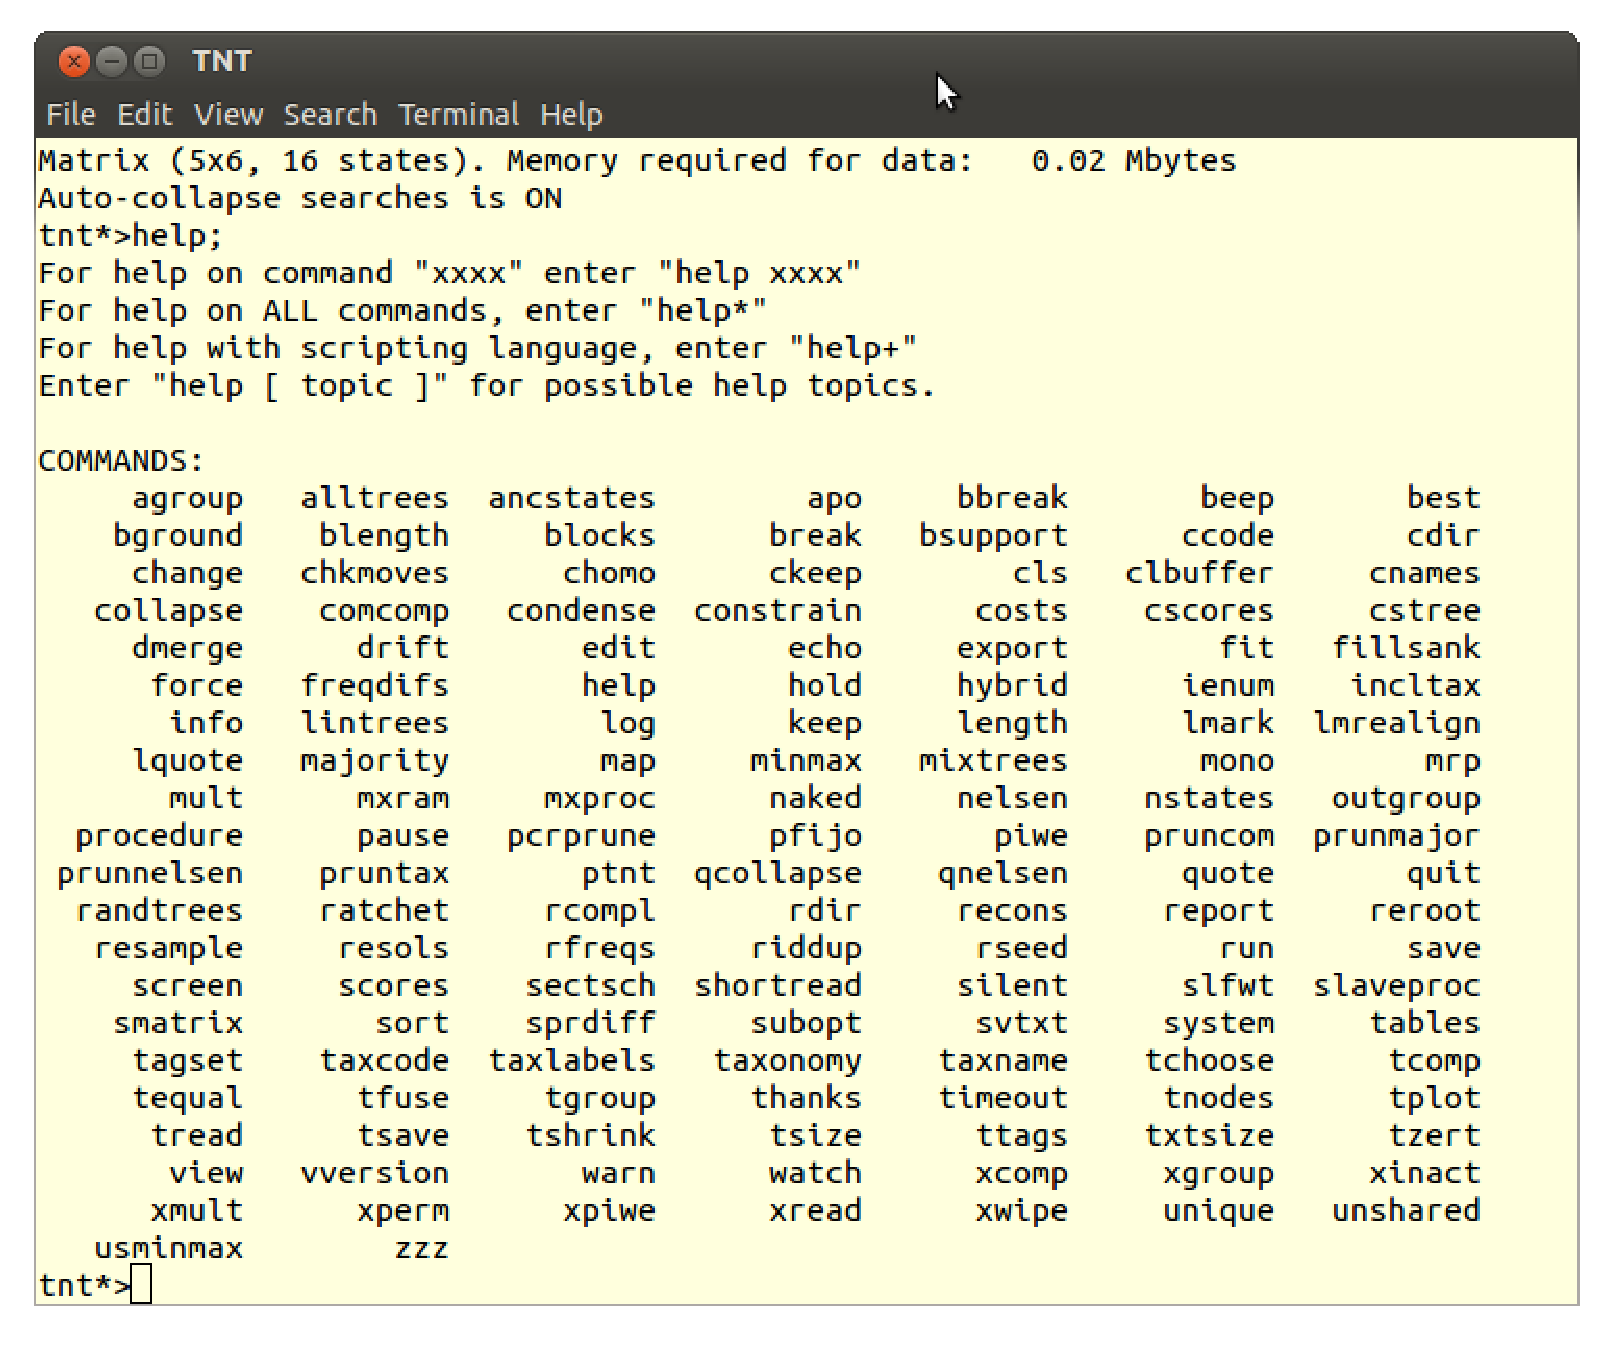
\includegraphics[scale=0.40]{figures/tut4/tnt_help.eps}}
      {\caption[\textit{\textit{Ajuda para comandos de TNT} }]{Lista de comandos disponíveis na documentação interna de TNT.}\label{tut4:fig:tnt_help}}
  \end{figure}

%%%%%%%%%%%%%%%%%%%%%%%%%%% FIM DA FIGURA FLAT %%%%%%%%%%%%%%%%%%%%%

Os detalhes desses comandos podem ser vistos executando ``\texttt{help nome\_do\_comando}'', como por exemplo ``\texttt{help collapse}'', ``\texttt{help proc}'' e ``\texttt{help zzz}''. O primeiro comando regula as regras de colapso de ramos (que discutiremos em momento oportuno), o segundo controla o direcionamento da entrada de comandos em TNT e o terceiro termina a seção de TNT. Execute esse último comando!\\

\section{Leitura de topologias em TNT}\label{tut4:tread}

Da mesma forma que o TNT lê matrizes de dados, o programa também permite ler e salvar tolopogias. Os arquivos de topologia também obecedem uma lógica, muito similar àquela utilizada nos arquivos que contém dados. Veja o exemplo abaixo:\\

\indent\indent\texttt{tread}\\
\indent\indent\texttt{'topologias para o exemplo\_1.tnt'}\\
\indent\indent\texttt{(taxon\_1 (taxon\_3 (taxon\_2 (taxon\_4 (taxon\_5 taxon\_6)))))* }\\
\indent\indent\texttt{(taxon\_1(taxon\_5(taxon\_3(taxon\_2(taxon\_4 taxon\_6)))))* }\\
\indent\indent\texttt{(taxon\_1 (taxon\_2 (taxon\_3 (taxon\_6 (taxon\_4 taxon\_5)))));}\\

A primeira linha deste arquivo deve conter o termo ``\texttt{tread}'', de \textit{tree read}, indicando ao TNT que ele deverá ler uma ou mais topologias. Na próxima linha você pode ou não inserir um comentário (\textit{e.g.}, ``\texttt{'topologias para o exemplo\_1.tnt'}''). A seguir você deve inserir a(s) topologia(s) em notação parentética obedecendo as seguinte regras:

\begin {myindentpar}{0.5cm}
\begin{enumerate}[\itshape a.]
	\item{Topologias que não sejam a última são seguidas de ``\texttt{*}''.}
	\item{A topologia final é seguida de ``\texttt{;}''.}
	\item{Terminais confinados a um conjunto de parênteses (\textit{i.e.}, ``\texttt{(taxon\_4 taxon\_6)}'') devem estar separados por um espaço.}
\end{enumerate}
\end{myindentpar}

\stepcounter{ex}
\begin{blackBlock}{\textbf{Exercicio 4.\arabic{ex}}}\label{tut4:ex:4.3}
	Neste exercício você deverá ler uma matriz e um conjunto de topologias e verificar o custo destas topologias.

\begin {myindentpar}{0.5cm}
\begin{enumerate}[\itshape a.]

	\item{Inicie o TNT};
	\item{Leia a matriz a ``\texttt{exemplo\_1.tnt}'' que você ditou no exercicio anterior};
	\item{Leia o arquivo ``\texttt{exemplo\_1.tre}'' da mesma forma que você leu a matriz de dados};
Observe que o TNT leu três topologias as quais foram atribuídas números de 0 a 2. Essa é outra peculiaridade de TNT, toda contagem se inicia em \textbf{0 (ZERO)} neste programa, \textbf{lembrem-se sempre desta particularidade do TNT!}
	\item{Consulte o \textit{help} para o comando ``\texttt{scores}'' e execute-o}.

\end{enumerate}
\end{myindentpar}

\end{blackBlock}

Ao final desse exercício você deverá ter obtido:\\

\begin{tabular}{ l c c c}
    & \texttt{0} & \texttt{1} & \texttt{2}\\
  \texttt{0} & \texttt{6} & \texttt{7} & \texttt{5}\\
\end{tabular}
\\

A primeira linha e a primeira coluna desta tabela impressa pelo TNT servem de referência para identificar a qual topologia o custo se refere. Por exemplo, a segunda linha e segunda coluna, onde se lê \texttt{6}, refere-se a topologia \texttt{00}; a segunda linha e terceira coluna, onde se lê \texttt{7}, refere-se a topologia \texttt{01}; finalmente, a segunda linha e quarta coluna, onde se lê \texttt{5}, refere-se a topologia \texttt{02}.

\stepcounter{ex}
\begin{blackBlock}{\textbf{Exercicio 4.\arabic{ex}}}\label{tut4:ex:4.4}
	Use o comando ``\textit{help}'' do TNT para o comando de linha ``\texttt{tchoose}''. Com base no conhecimento sobre o TNT que você obteve até este momento, você deverá manter apenas a topologia mais curta na memória do TNT e posteriormente imprimí-la na tela de seu computador. Quais foram os comandos que você executou para cumprir estas tarefas?
 \begin{center}
  \line(1,0){400}\\
  \line(1,0){400}\\
 \end{center}

\end{blackBlock}

\stepcounter{ex}
\begin{blackBlock}{\textbf{Exercicio 4.\arabic{ex}}}\label{tut4:ex:4.5}
	Neste exercício, você deverá editar manualmente o arquivo ``\texttt{exemplo\_1.tre}''. Você deverá criar uma topologia qualquer, diferente das demais, na última linha do arquivo -- ou seja, topologia ``\texttt{3}''. Posteriormente, você deverá salvar o arquivo editado sob o nome de ``\texttt{exercicio\_1b.tre}''. Abaixo, ilustre todas as topologias neste arquivo, bem como seus respectivos custos e indique os comandos utilizados para completar o exercício. 

\vspace{120pt}

 \begin{center}
  \line(1,0){400}\\
  \line(1,0){400}\\
 \end{center}

\end{blackBlock}


\section{Como salvar topologias em TNT}\label{tut4:tsave}
O TNT salva topologias em 3 formatos. No primeiro deles, \textit{default} de TNT, as topologias são salvas em formato binário. Arquivos binários são aqueles que só podem ser interpretados por programas e/ou processadores. Desta forma, embora este formato seja apropriado para gerar arquivos pequenos com muito conteúdo -- topologias -- ele só será lido em TNT. Os demais formatos usados pelo TNT para salvar topologias geram arquivos textos. Estes tem a vantagem de poderem ser lidos por outros programas -- algumas vezes com pequenas modificações -- e/ou examinados em editores de texto. Isso é muito vantajoso, embora o custo evidente é que os arquivos são maiores que aqueles gerados no formato binário. A seguir iremos ver as diferenças entre esses dois formatos.\\

\stepcounter{ex}
\begin{blackBlock}{\textbf{Exercicio 4.\arabic{ex}}}\label{tut4:ex:4.6}
	Neste exercício, iremos explorar duas formas de salvar topologias em TNT e verificar no que eles diferem.

\begin {myindentpar}{0.3cm}
\begin{enumerate}[\itshape i.]

	\item{Abra o arquivo \texttt{exemplo\_2.tnt} e execute uma busca por \textit{implicit enumeration}. Você deverá obter 2 topologias com o custo de 6 passos.}
	\item{Execute os seguintes comandos: ``\texttt{tsave* exercicio\_2a.tre;}'', ``\texttt{save;}'', e ``\texttt{tsave/;}''}
	\item{Execute os seguintes comandos: ``\texttt{taxname =;}'', ``\texttt{tsave* exercicio\_2b.tre;}'', ``\texttt{save;}'', e ``\texttt{tsave/;}''}
	\item{Consulte o ``\textit{help} do TNT e anote a função de cada comando utilizado nas linhas abaixo:}

Comandos:\\
\texttt{taxname =}:~~\line(1,0){320}\\
\texttt{tsave*}:~~~~~~~~~\line(1,0){320}\\
\texttt{save}:~~~~~~~~~~~~~~\line(1,0){320}\\
\texttt{tsave/}:~~~~~~~~~\line(1,0){320}\\
	\item{Verifique os conteúdos dos arquivos \texttt{exercicio\_2a.tre} e \texttt{exercicio\_2b.tre} e responda: Qual é a diferença entre eles?}
\begin{center}
\line(1,0){400}\\
\line(1,0){400}\\
\end{center}
\end{enumerate}
\end{myindentpar}

\end{blackBlock}


\section{Busca de topologias em TNT}\label{tut4:search}

Algoritmos de busca podem ser exatos ou heurísticos. Algorítmos exatos, sejam eles por enumeração implícita ou explícita \parencite{Land_and_Doig_1960, Hendy_and_Penny_1982}, avaliam todo o espaço de solução -- no nosso caso o espaço de topologias --, e garantem que a solução ótima para a sua matriz (\textit{i.e.}, menor custo) foi encontrada. Algoritmos heurísticos, não lhe fornecem esta garantia, pois examinam uma amostra do seu espaço de topologias. Desta forma, poderíamos pensar de imediato que sempre deveríamos escolher algoritmos exatos. No entanto, como vocês verão, há limitações quanto ao uso desses algoritmos em inferência filogenética.

TNT possui um algoritmo de busca exata por enumeração implícita. Enumeração implícita significa que ``implicitamente'' o algoritmo examinou todas as topologias que potenciamente poderiam ter um custo menor do que uma aproximação inicial -- como discutimos na aula teórica. Vejamos algumas propriedades destes algoritmos.\\

\stepcounter{ex}
\begin{blackBlock}{\textbf{Exercicio 4.\arabic{ex}}}\label{tut4:ex:4.7}
	Considere os arquivos da Tabela \ref{tut4:table:ie}. Para cada um deles, execute uma busca com o algoritmo ``\texttt{ie}'', registre o tempo de execução da análise na Tabela \ref{tut4:table:ie} e responda: 

\begin {myindentpar}{0.5cm}
\begin{enumerate}[\itshape a.]
	\item{Quais são as diferenças entre estas matrizes de dados?}
\begin{center}
\line(1,0){400}\\
\line(1,0){400}\\
\end{center}

	\item{O que acontece com o tempo de execução da análise em relação às diferenças observadas nestes arquivos?}
\begin{center}
\line(1,0){400}\\
\line(1,0){400}\\
\end{center}

	\item{O que impede o uso deste algorítmo em análises filogenéticas?}
\begin{center}
\line(1,0){400}\\
\line(1,0){400}\\
\end{center}

\end{enumerate}
\end{myindentpar}

\end{blackBlock}

%%%%%%%%%%%%%%%%%%%%%%%%%%% TABELA DE PARA IMPLICIT ENUMERATION %%%%%%%%%%%%%%%%%%%%%%%%%%% 
%\begin{landscape}
\pagestyle{fancy}
\begin{center}

\begin{longtable}{lcccccc}
\caption[Tabela \ref{tut4:table:ie}: Templo de execução em \textit{implicit enumeration}]{Templo de execução em \textit{implicit enumeration}.} \label{tut4:table:ie} \\


\hline\hline \textbf{Matriz de dados} & \textbf{Tempo}\\
\endfirsthead

\multicolumn{6}{c}{{\bfseries \tablename\ \thetable{} -- Continuação.}}\\
\hline\hline \textbf{Matriz de dados} & \textbf{Tempo}\\
\endhead
%\hline \multicolumn{6}{r}{{--continua na próxima página}} \\ \hline
%\endfoot
\hline \hline
%\hline \multicolumn{6}{l}{Consulte a página \url{http://wiki.linuxquestions.org/wiki/Linux_software_equivalent_to_Windows_software}.}
\endlastfoot
\hline
\texttt{10x500.tnt} & ~~~~~~~~~~~~~~~~~~~~~~~~\\
\texttt{10x1000.tnt} & ~~~~~~~~~~~~~~~~~~~~~~~~\\
\texttt{10x1500.tnt} & ~~~~~~~~~~~~~~~~~~~~~~~~\\
\texttt{15x500.tnt} & ~~~~~~~~~~~~~~~~~~~~~~~~\\

\end{longtable}
\end{center}
%\end{landscape}

%%%%%%%%%%%%%%%%%%%%%%%%%%% FIM DA TABELA IE %%%%%%%%%%%%%%%%%%%%%%%%%%


Deve ter ficado claro que o número de terminais limita o uso de buscas exatas. A busca por topologias ótimas não é tarefa trivial, principalmente pelo fato de que o número de topologias possíveis cresce exponencialmente à medida em que adicionamos terminais -- como vimos anteriormente (veja Tutorial \ref{tut3}). Mesmo algoritmos que utilizam enumeração implícida, no qual grande parte do universo de topologias possíveis é descartada, o tempo computacional pode ser muito alto. Desta forma, métodos heurísticos são frequentemente utilizados para esse propósito.

%%%%%%%%%%%%%%%%%%%%%%%%%%% FIGURA FLAT %%%%%%%%%%%%%%%%%%%%%%%%%%%
%  \vspace{-1em}
  \begin{figure}[H]
    %\ffigbox[\FBwidth]
       \centering
      {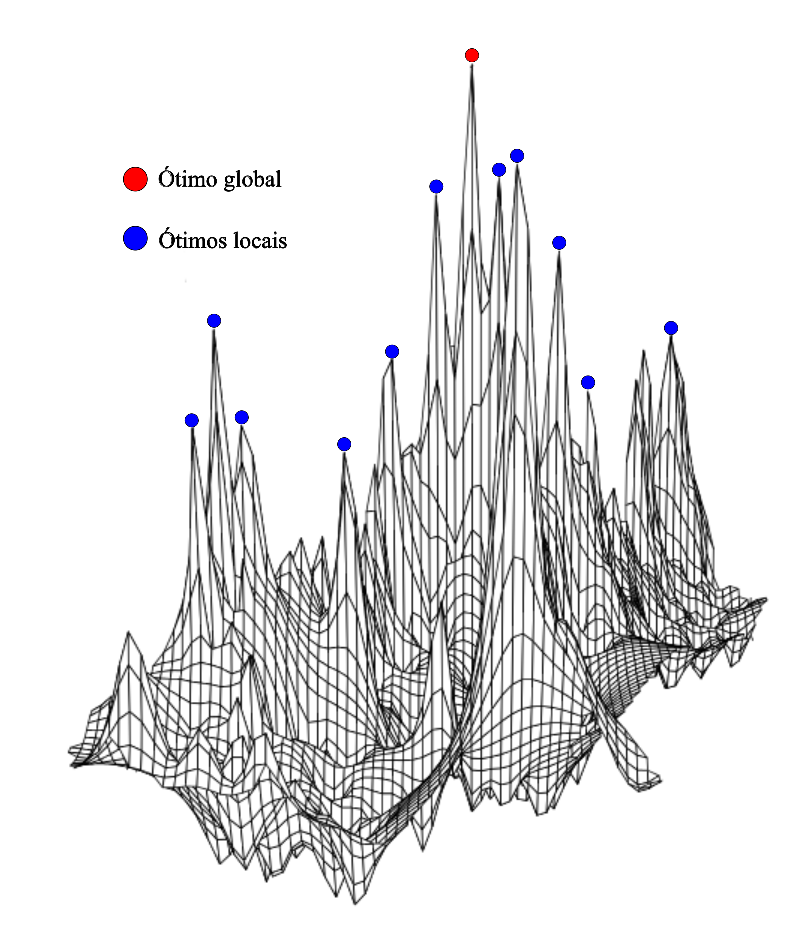
\includegraphics[scale=0.70]{figures/tut4/landscape.eps}}
      {\caption[\textit{\textit{Ótimos locais e globais} }]{Ótimos locais e globais representados em uma superfície de relevo.}\label{tut4:fig:landscape}}
  \end{figure}

%%%%%%%%%%%%%%%%%%%%%%%%%%% FIM DA FIGURA FLAT %%%%%%%%%%%%%%%%%%%%%



O desafio de métodos heurísticos é explorar o espaço de topologias o suficiente para evitar ficar restrito a ótimos locais (Figura \ref{tut4:fig:landscape}). A analogia geralmente utlizada para explicar o conceito de ótimos locais e global é ilustrada no relevo representado na Figura \ref{tut4:fig:landscape}. Este relevo indica um pico mais alto que os demais (em vermelho) quee representaria a solução ótima -- \textit{i.e.}, a(s) topologia(s) mais curta(s). O relevo inclui ainda uma série de outros picos menores que representam uma ou mais topologias sub-ótimas. O objetivo destes algoritmos é evitar ficar trancados em ótimos locais -- o que depende do quão eficientemente ele explora o espaço de topologias. Vale ressaltar que a complexidade deste relevo depende de vários fatores, tais como o número de soluções possíveis -- que determina e espaço e o incremento de distâncias topológicas -- e estruturação dos dados (veja Tutorial \ref{tut3}).

Dentro do que é conhecido como  busca por trajetória (\textit{trajectory search}), a grade maioria dos algoritmos heurísticos inicia sua busca construindo uma árvore de Wagner \parencite{Wagner_1961}, em uma etapa conhecida como \textit{random addition sequence} (\textbf{RAS}). Após a construção inicial, a árvore de Wagner é submetida a algoritmos de refinamento por um procedimento conhecido como \textit{branch swapping}. Neste contexto, a árvore de Wagner determina um ponto inicial neste espaço e os procedimentos de refinamento asseguram a melhor solução local. Dentre estes algoritmos de \textit{branch swapping} mais comumente implementados, podemos citar \textit{nearest-neighbor interchange} \parencite[\textbf{NNI}, ][]{Camin_and_Sokal_1965, Robinson_1971}, \textit{Tree-Bisection and Regrafting} \parencite[TBR, ][]{Swofford_1990} ou ``\textit{Branch-Breaking}'' \parencite[][]{Farris_1988}. Estes algoritmos estão virtualmente implementados em todos os programas de inferência filogenética, incluindo TNT. Detalhes sobre esses algoritmos podem se encontrados em \parencite{SwoffordEtAl1996, Page_and_Homes_1998, Schuh_2000, Felsenstein_2004, Giribet_2007}.

\stepcounter{ex}
\begin{blackBlock}{\textbf{Exercicio 4.\arabic{ex}}}\label{tut4:ex:4.8}
	Neste exercício vamos explorar os algoritmos de buscas por trajetória  existentes no TNT. Considere o arquivo \texttt{zilla.tnt}. Este arquivo contém 500 terminais, o que torna impraticável o uso de algoritmos exatos. Veremos o comportamento de TNT em relação aos parâmetros de análises de buscas heurísticas simples (\textit{i.e., traditional search}). 
%\end{blackBlock}

	\begin {myindentpar}{0.3cm}
	\begin{enumerate}[\itshape i.]
		\item{Reinicie o TNT para nos certificarmos de que estamos usando os parâmetros de \textit{default} do programa.}
		\item{Leia o arquivo \texttt{zilla.tnt} em TNT}.
		\item{O algoritmo de busca tradicional do TNT inclui \textbf{N} adições aleatórias (\textbf{RAS}) que controem árvores de Wagner seguidas de refinamento por SPR e/ou TBR. O comando para sua execução é ``\texttt{mu}'' e para saber quais são os parâmetros de \textit{default} deste comando você deve executar o comando ``\texttt{mu:;}''}. Execute este último comando e anote os parâmetros abaixo:\\

	\texttt{Settings for multiple random addition sequences:}\\
	\indent\indent\texttt{ * \_\_ random sequences}\\
	\indent\indent\texttt{ * saving up to \_\_ trees per replication}\\
	\indent\indent\texttt{ * swapping trees with \_\_}\\
	\indent\indent\texttt{ * keeping only the best trees found }\\

		\item{Execute o comando ``\texttt{mu}'' e verifique o resultado impresso no terminal. Você deverá ter obtido um resultado muito semelhante àquele ilustrado na Figura \ref{tut4:fig:tnt_mu}.}

	%%%%%%%%%%%%%%%%%%%%%%%%%%% FIGURA MU %%%%%%%%%%%%%%%%%%%%%%%%%%%
	%  \vspace{-1em}
	  \begin{figure}[H]
	    %\ffigbox[\FBwidth]
             \centering
	      {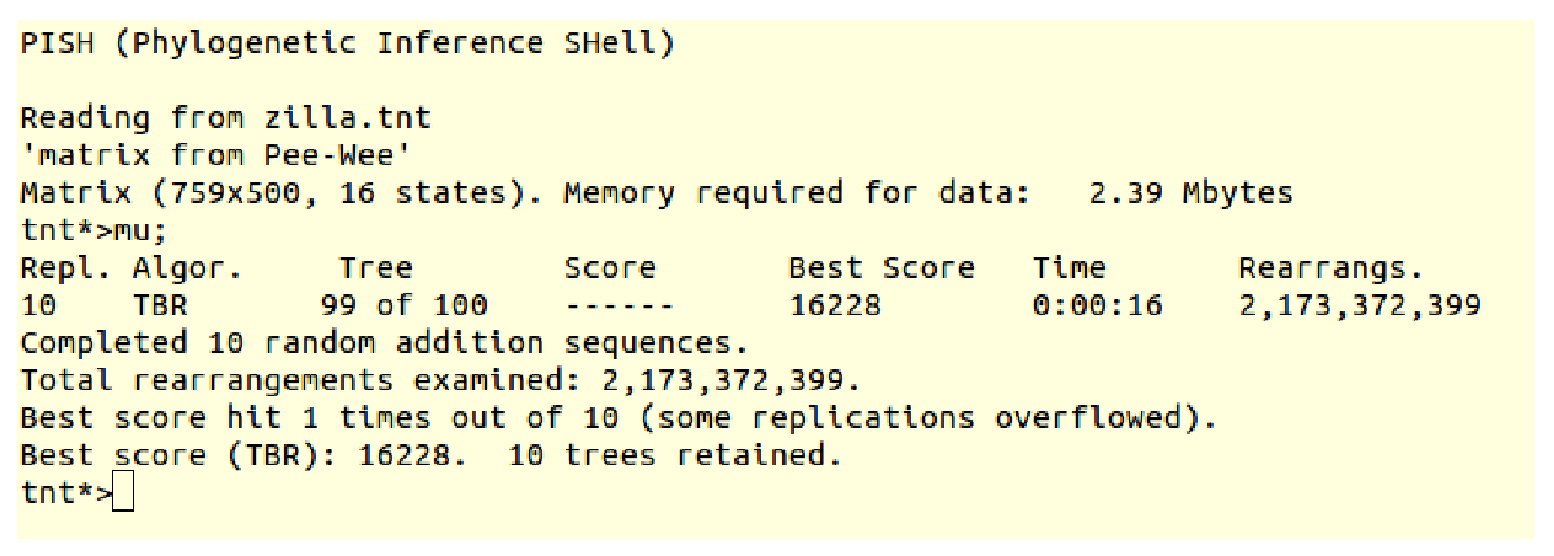
\includegraphics[scale=0.50]{figures/tut4/tnt_mu.eps}}
	      {\caption[\textit{\textit{Resultado de busca heurística em TNT} }]{Resultado de busca em TNT utilizando os parâmetros de \textit{default} do comando \texttt{mu}.}\label{tut4:fig:tnt_mu}}
	  \end{figure}

	%%%%%%%%%%%%%%%%%%%%%%%%%%% FIM DA FIGURA MU %%%%%%%%%%%%%%%%%%%%%

O resultado informa que foram feitas 10 réplicas (\textbf{RAS}) e que as topologias mais curtas possuíam 16228 passos, que esse custo foi obtido em apenas uma réplica (\textit{i.e.}, ``\texttt{Best score hit 1 times}'') e que foram retidas 10 topologias na memória (\textit{i.e.}, ``\texttt{10 trees retained}''). Observe que o TNT informa quantas topologias foram examinadas, o tempo de execução, e que durante a busca, algumas réplicas excederam o número de topologias que poderia ser mantida (\textit{i.e.}, ``\texttt{some replications overflowed}'').

Você consideraria que esses parâmetros configuram uma boa estratégia de busca heurística para esses dados? Saiba que para esta matriz há pelo menos 46 topologias com o custo de 16218 passos! Você terá muita sorte se conseguir atingir esse resultado utilizando esses algoritmos, principalmente com os parâmetros iniciais.

\item{Há vários parâmetros que controlam a qualidade de buscas heurísticas, vejamos como controlá-los:}

\subitem{\textbf{replic:}} Essa opção é a mais óbvia de todas, pois ela controla o número de adições aleatórias do comando ``\texttt{mu}'' (\textit{ex.} \texttt{mu: rep 100}).

\subitem{\textbf{hold:}} Possui duas funções. Como \textbf{comando} de TNT ele controla o número máximo de topologias que o TNT irá manter na memória. Seu valor de \textit{default} é 100. Portanto, ao chegar a esse valor o TNT interrompe a busca! Como \textbf{opção} do comando ``\texttt{mu}'', ``\texttt{hold}'' controla o número máximo de topologias que será mantida durante cada réplica.

É necessário manter um balanço entre o comando ``\texttt{hold}'' e as opções de ``\texttt{mu}''. Por exemplo, se você modificar o número de réplicas em ``\texttt{mu}'' utilizando o comando `\texttt{mu: rep 100}, ao executar a busca o TNT irá interrompê-la na décima réplica e retornará a seguinte mensagem: ``\texttt{NOTE: Search terminated after replication 10 (tree buffer full)}''. Isso ocorre porque havia espaço para 100 topologias na memória do TNT e a busca por ``\texttt{mu}'' estava configurada para manter apenas 10 topologias por réplicas. Portanto, 10 x 10 = 100! Fim. Desta forma, o número de topologias atribuídas ao \textbf{comando} ``\texttt{hold}'' deve ser maior ou igual ao número atribuído à \textbf{opção} ``\texttt{hold}'' de ``\texttt{mu}'' vezes o número de réplicas. Entender os conceitos associados a esse balanço é muito importante.

\subitem{\textbf{mxram:}} Por \textit{default}, o TNT aloca 16 MB de memória para si. No entanto, esse número pode ser insuficiente para algumas análises uma vez que ele influencia diretamente o número de topologias que o TNT poderá manter na memória. Por exemplo, se você digitar o comando hold no \textit{prompt} do TNT saberá quantas topologias ele irá manter durante sua busca. Tente modificar esse número para 1000 (\textit{i.e.}, \texttt{hold 1000;}). Você não deve ter tido nenhum problema, mas se tentar modificar para 10000 verá que o TNT não poderá fazê-lo. No entanto, se você alocar mais memória ao TNT, \textit{i.e.}, ``\texttt{mxram 512;}'' isso será possível. \textbf{Um detalhe, quando ``mxram'' é modificado, o TNT requer que você leia seus dados novamente!}

\subitem{\textbf{Algoritmos de refinamento:}} Por \textit{default}, o TNT utiliza TBR após a construção de árvores de Wagner ao invés de SPR. O TBR é um algoritmo mais agressivo de refinamento (\textit{branch swapping}), porém sua complexidade possui uma função cúbica ao passo que SPR possui uma complexidade quadrática. Portanto, a complexidade desses algoritmos tem influência direta no tempo de execução. Considere que SPR é um subconjunto das topologias examinadas por TBR.

\item{Antes de passar para o próximo exercício, manipule esses comandos e opções para que você tenha uma ideia melhor de como o TNT pode ser controlado.}

	\end{enumerate}
	\end{myindentpar}

\end{blackBlock}




\stepcounter{ex}
\begin{blackBlock}{\textbf{Exercicio 4.\arabic{ex}}}\label{tut4:ex:4.9}

Neste último exercício, você deverá conceber um experimento de 15 a 20 execuções de TNT usando a matriz em \texttt{zilla.tnt} variando o número de adições aleatórias e o número de topologias mantidas em cada uma das réplicas. Seu objetivo é conceber um desenho experimental no qual você possa avaliar como esses dois parâmetros afetam a eficiências de sua análise. A eficiência deve ser medida pelo tempo necessário para obter o menor custo e o número de topologias recuperadas. Para cada execução você deverá registrar os dados na Tabela \ref{tut4:table:mu} abaixo. Executado o experimento, responda:

	\begin {myindentpar}{0.5cm}
	\begin{enumerate}[\itshape a.]
		\item{Você consegue enxergar algum padrão que lhe indique alguma estratégia eficiente de busca? Qual seria?}
	\begin{center}
	\line(1,0){400}\\
	\line(1,0){400}\\
	\line(1,0){400}\\
	\end{center}

		\item{Você conseguiu obter topologias com custo igual o inferior a 16218? Caso não tenha conseguido, qual seria sua estratégia para chegar a esse custo?}
	\begin{center}
	\line(1,0){400}\\
	\line(1,0){400}\\
	\line(1,0){400}\\
	\end{center}


	\end{enumerate}
	\end{myindentpar}

\end{blackBlock}

Há três \textit{scripts} no diretório deste tutorial sob a extensão \texttt{*.run} que podem automatizar a execução desse exercício. Em comum, esses \textit{scripts} executam o TNT em uma série de vezes e registra os resultados em um arquivo texto. A explicação de um deles será suficiente para que você entenda a lógica dos demais. Considere o conteúdo do arquivo \texttt{mu\_hold.run}:

\begin{lstlisting}[label=tut4:tnt_macro]
mxram 512;
macro =;
proc zilla.tnt
hold 10000;
log mu_hold.txt;
loop 10+1 20
    mu: rep 5 hold #1;
    mu;
stop
log/;
macro -;
zzz
\end{lstlisting}


Neste \textit{script} -- ou macro de TNT, a primeira linha (1) aloca 512M de memória para o programa -- o que é desejável em muitos casos, pois isso lhe permite acumular mais topologias durante a execução do programa. A segunda linha habilita a linguagem do macro de TNT. Macros funcionam como uma linguagem interna que lhe permite fazer algumas operações que seus comandos gerais não permitem, como por exemplo \textit{loops} -- veja abaixo. Na terceira linha, o TNT é instruido a ler a matriz \texttt{zilla.tnt}. A linha 4 define o número máximo de topologias que o TNT poderá manter na memória. Até aqui, não há novidades, o mais interessante começa agora. Na linha 5, o \textit{script} abre um arquivo de log. O log do TNT permite que tudo que é impresso no console do programa durante sua execução seja também direcionado para um arquivo texto. Isso pode ser desejável se você precisa coletar informações de execuções longas ou mesmo documentar o que fez. Na linha 10, esse arquivo de log é fechado. Portanto, tudo que ocorrer entre as linhas 6 e 9 será automaticamente gravado no arquivo \texttt{mu\_hold.txt}. A linha 6 implementa um comando de macro denominado \texttt{loop}. Como o próprio nome sugere, esse comando abre um ciclo de execuções. Este ciclo começa no 10 e termina no 20 em intervalos de 1, portando ``$10+1~~~20$''. Na linha 7, a variável ``$\#1$'' receberá o valor da contagem de cada \texttt{loop} para definir os parâmetros de \texttt{mu}. Desta forma, no primeiro \texttt{loop} a linha 7 será ``\texttt{mu: rep 5 hold 10}'', no segundo ``\texttt{mu: rep 5 hold 11}'', no terceiro ``\texttt{mu: rep 5 hold 12}'', etc -- até  ``\texttt{... hold 20}''. Para cada modificação da linha 7, o TNT executa a busca heurística pelo comando ``\texttt{mu}''. Ao final (\textit{e.i.}, \texttt{hold 20}) o \texttt{loop} é finalizado (lina 9), o log é fechado (linha 10), a linguagem macro é desabilitada (linha 11) e o TNT é fechado. Se você examinar os outros dois arquivos com a extensão \texttt{*.run} verá que eles obedecem a mesma lógica. Você pode mudar os valores do loop como quiser ou até mesmo implementar outros comandos de TNT dentro e fora do \texttt{loop}. Bom exercício!




%%%%%%%%%%%%%%%%%%%%%%%%%%% TABELA DE PARA BUSCAS HEURÍSTICAS %%%%%%%%%%%%%%%%%%%%%%%%%%% 
%\begin{landscape}
\pagestyle{fancy}
\begin{center}

\begin{longtable}{|c|c|c|c|c|c|c}
\caption[Tabela \ref{tut4:table:mu}: Buscas heurísticas em TNT]{Número de sequências aleatórias (\textbf{RAS}), topologias mantidas em cada réplica, número de topologias examinadas, tempo de execução, número de \textit{hits} no menor custo e custo encontrado para buscas heurísticas utilizando a matriz zilla.tnt.} \label{tut4:table:mu} \\


\hline\hline \textbf{RAS} & \textbf{Trees/RAS} & \textbf{\# Rearrangements} & \textbf{Time} & \textbf{\# Hits Best} & \textbf{Best Score}\\
\endfirsthead

\multicolumn{6}{c}{{\bfseries \tablename\ \thetable{} -- Continuação.}}\\
\hline\hline \textbf{RAS} & \textbf{Trees/RAS} & \textbf{\# Rearrangements} & \textbf{Time} & \textbf{\# Hits Best} & \textbf{Best Score}\\
\endhead
%\hline \multicolumn{6}{r}{{--continua na próxima página}} \\ \hline
%\endfoot
\hline \hline
%\hline \multicolumn{6}{l}{Consulte a página \url{http://wiki.linuxquestions.org/wiki/Linux_software_equivalent_to_Windows_software}.}
\endlastfoot
\hline~&~&~&~&~&~\\
\hline~&~&~&~&~&~\\
\hline~&~&~&~&~&~\\
\hline~&~&~&~&~&~\\
\hline~&~&~&~&~&~\\
\hline~&~&~&~&~&~\\
\hline~&~&~&~&~&~\\
\hline~&~&~&~&~&~\\
\hline~&~&~&~&~&~\\
\hline~&~&~&~&~&~\\
\hline~&~&~&~&~&~\\
\hline~&~&~&~&~&~\\
\hline~&~&~&~&~&~\\
\hline~&~&~&~&~&~\\
\hline~&~&~&~&~&~\\
\hline~&~&~&~&~&~\\
\hline~&~&~&~&~&~\\
\hline~&~&~&~&~&~\\
\hline~&~&~&~&~&~\\
\hline~&~&~&~&~&~\\
\hline~&~&~&~&~&~\\
\hline~&~&~&~&~&~\\

\end{longtable}
\end{center}
%\end{landscape}

%%%%%%%%%%%%%%%%%%%%%%%%%%% FIM DA TABELA PARA BUSCAS HEURÍSTICAS %%%%%%%%%%%%%%%%%%%%%%%%%%


%%%%%%%%%%%%%%%%%%%%%%%%%%%% HERE ENDS TEXT AND ADDS REFERENCES %%%%%%%%%%%%%%%%%%%%%%%%%%%% 
\section{Referências}\label{tut4:refs}
\printbibliography[heading=none]
\end{refsection}
%

